\section{CONCLUSIONS}
In this paper, we proposed a methodology of multiple objects transportation by the transformable multirotor with two-dimensional multilinks. We then described the form optimization method to obtain the optimal form based on the flight stability, along with the definition of the flight stability and constraints of forms to avoid invalid forms. We then developed the hardware and software system, including the multi-layer structure for internal communication. Finally, we showed the effectiveness of the proposed method by an experiment. In the experiment, we show the achievement of aerial transformation and multiple objects transportation.
\par
For future work, we will construct more rigid link module to achieve the aerial transformation with yaw control. Next, while the optimal form was calculated in off-line in this work, we will calculate that in on-line by estimating the weight of target objects based on change of the lifting force. Then, we must accelerate the calculation of the form optimization. Moreover, we are interested in multiple objects transportation by using whole-body aerial manipulation\cite{ZhaoICRA2017}, in which it is appeared that eight or more links are necessary.
%\begin{figure}[H]
%  \begin{center}
%    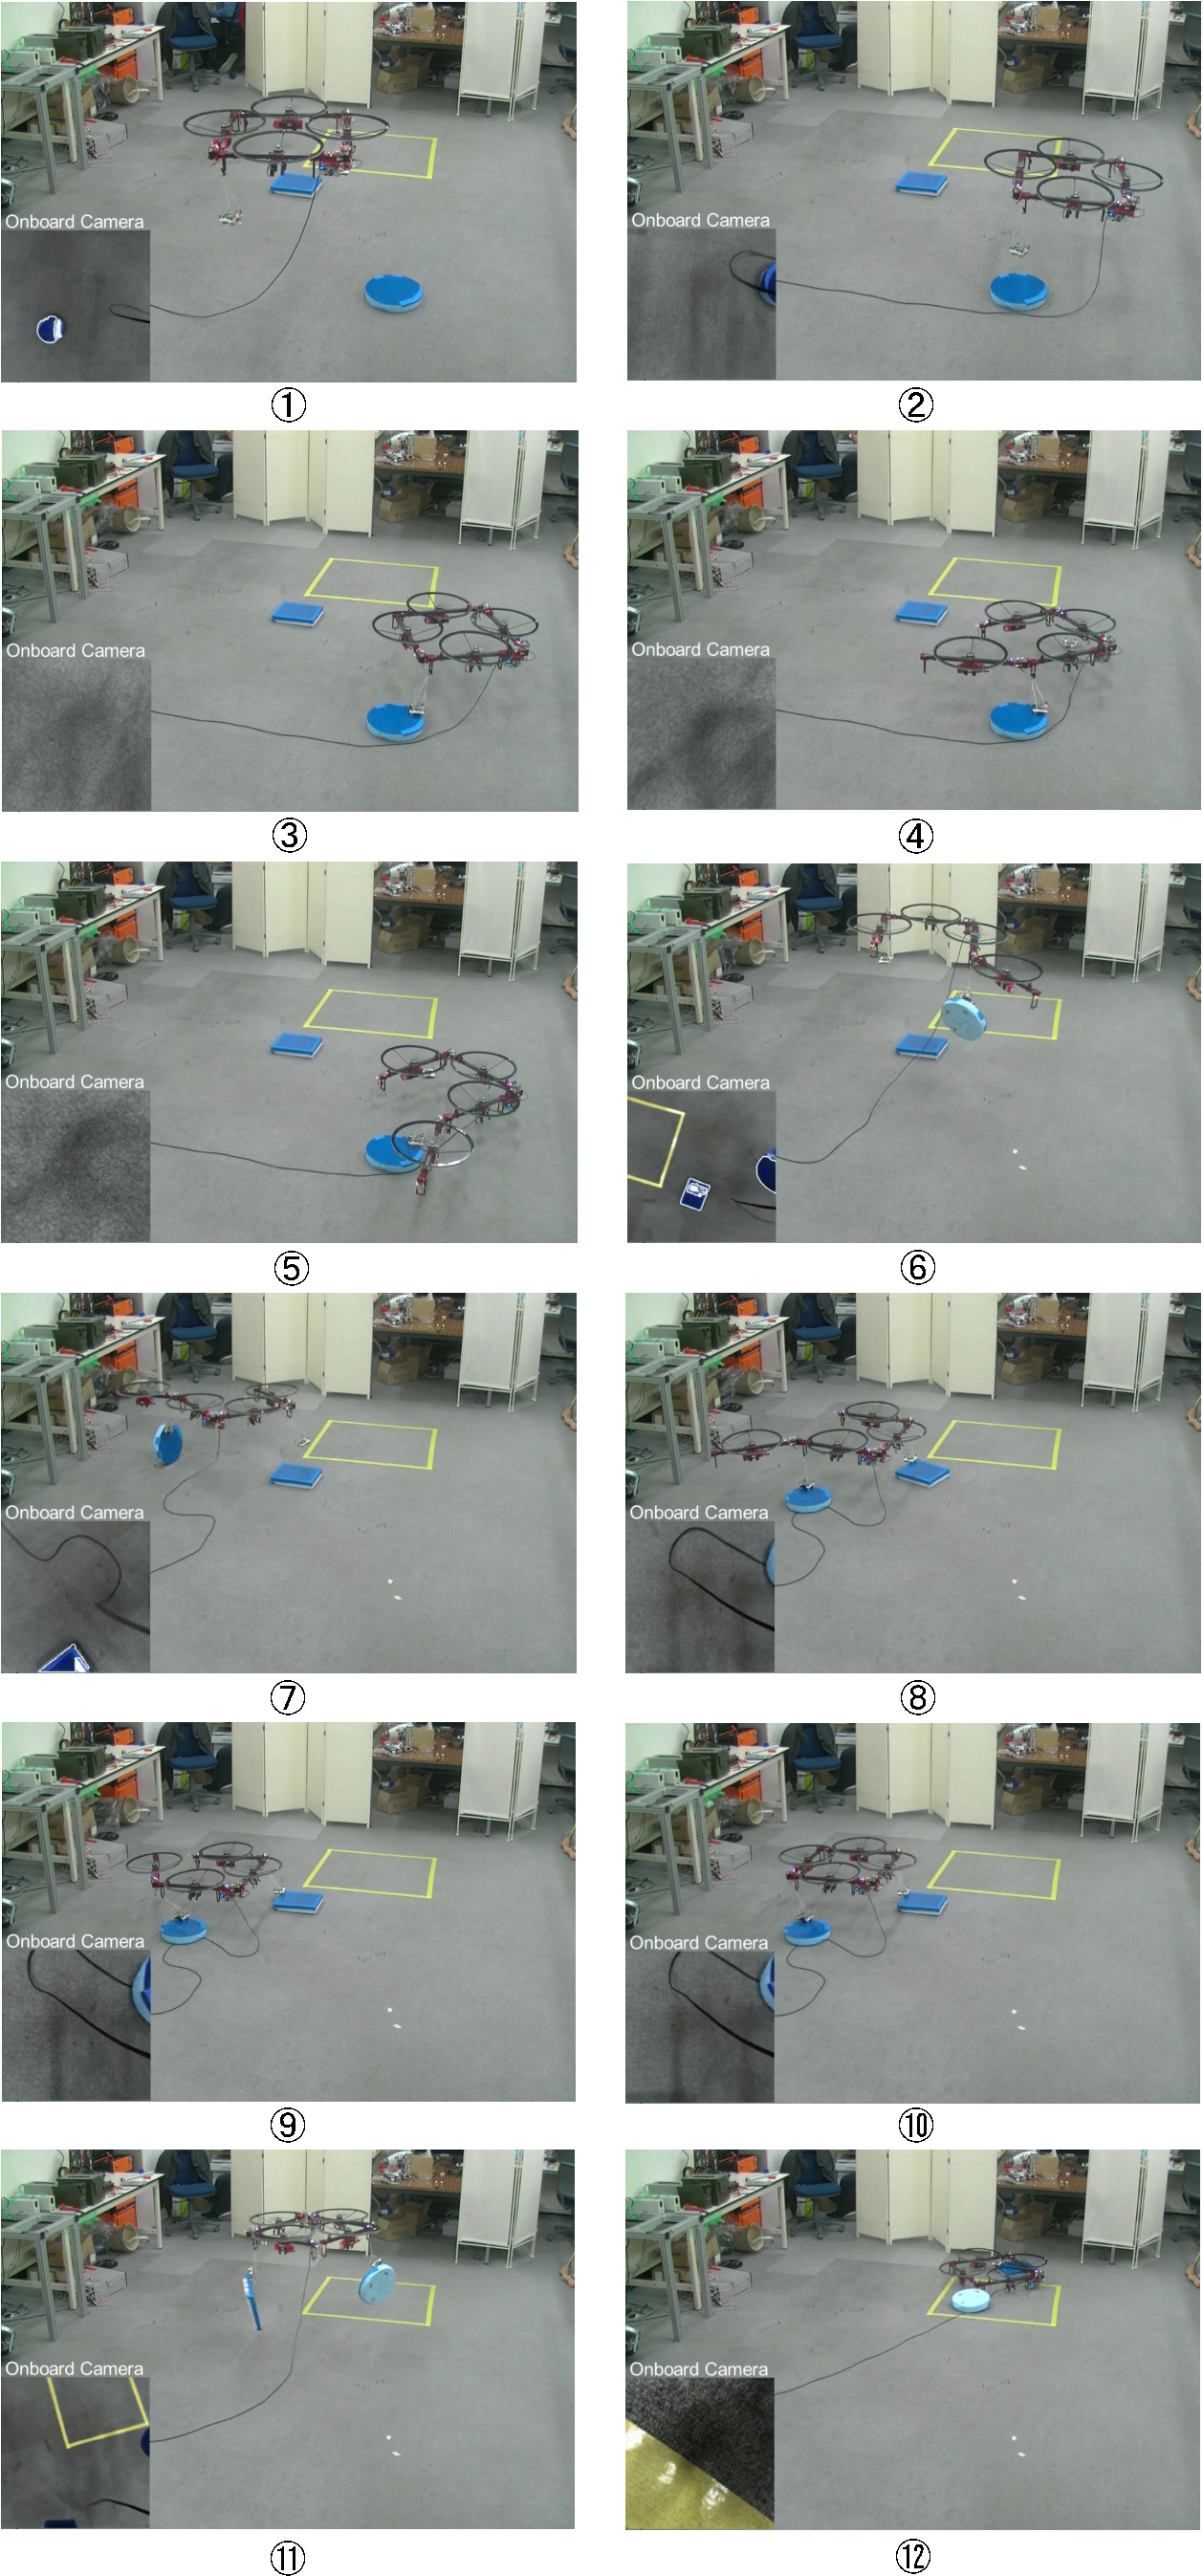
\includegraphics[width=1.0\columnwidth]{figs/experiment.pdf}
%  \end{center}
%  \caption{Experiment of multiple objects transportation: two ferrous objects are grasped and transported by the transformable aerial robot.\label{figure:experiment}}
%\end{figure}
